\section{Preliminaries}

Here, $\log n$ denotes the base two logarithm of $n$, for any natural number $n$.

\subsection{Complexity}

Here is a brief summary of the definitions of the complexity classes that appear in this paper.

\begin{itemize}
\item
  $\L$ is the class of languages decidable by a deterministic Turing machine that uses $O(\log n)$ space on inputs of length $n$.
  $\L^2$ is similar, but with $O(\log^2 n)$ space.
\item
  $\NL$ is the class of languages decidable by a nondeterministic Turing machine that uses $O(\log n)$ space.
  Equivalently, this is the class of languages $L$ for which there is a deterministic Turing machine with a two-way read-only tape for the input string, a one-way read-only tape for the nondeterministic bits, and a two-way read-write work tape in which only $O(\log n)$ cells are used, such that $x \in L$ if and only if there is a binary string $w$ of polynomial length such that the machine accepts on input $x$ and nondeterministic bits $w$.
\item $\NL[\log^2 n]$ is the subclass of $\NL$ in which the length of $w$ is bounded by $O(\log^2 n)$.
\item $\bL$ is the superclass of $\NL[\log^2 n]$ in which the machine has two-way access to the tape containing the nondeterministic bits.
  Equivalently, this is the class of languages $L$ such that there is a language $L' \in L$ such that $x \in L$ if and only if there is a binary string $w$ of length $O(\log^2 n)$ such that $(x, w) \in L'$.
\item
  $\FOLL$ is the class of languages decidable by a $\L$-uniform family of circuits with polynomial size, unbounded fan-in, and $O(\log \log n)$ depth.
  $\bFOLL$ is the class of languages decidable by $\FOLL$ circuits that have been augmented with $O(\log^2 n)$ nondeterministic bits (gates with no inputs and one output).
\item
  $\AC^0$ and $\bAC^0$ are the restrictions of $\FOLL$ and $\bFOLL$, respectively, to depth $O(1)$.
  $\NAC^0$ allows a polynomial number of nondeterministic bits.
\end{itemize}
In general, the class $\beta_2 \mathcal{C}$ is the class of languages decidable by $\mathcal{C}$ machines augmented with $O(\log^2 n)$ bits of nondeterminism, or equivalently, the class of languages verifiable by $\mathcal{C}$ machines when given a certificate of length $O(\log^2 n)$.

If $L_1$ and $L_2$ are languages, there is a \emph{logarithmic space many-one reduction} from $L_1$ to $L_2$, denoted $L_1 \leq_m^{\L} L_2$, if there is a function $f$ such that $f$ is computable in logarithmic space and $x \in L_1$ if and only if $f(x) \in L_2$.
%%\todo{CORRECT THIS DEFINITION to be more clear about nondeterministic function outputs (exists/forall)}
%% SHOWS UP IN A LATER SECTION \todo{Does Immerman-Szelpcsenyi Theorem apply to $\bL$?}
%% NO It seems not, since it would require guessing up to m shortcut edges. \todo{Is directed planar graph reachability in $\beta \L$? In $\NL[\log^{O(1)} n]$? See ``shortcut graphs'' by Thorup.}
%% \todo{Explain why the closure of L under beta AC reductions is probably not NL[log2 n], and maybe prove it?.}
There is a \emph{$\bAC^0$ conjunctive truth-table reduction} from $L_1$ to $L_2$, denoted $L_1 \leq^{\bAC^0}_{ctt} L_2$, if there is a function $f$ and a polynomial $p$ such that
\begin{itemize}
\item $f$ is computable in $\AC^0$,
\item $x \in L_1$ if and only if there is a $w$ of length $O(\log^2 n)$ such that $\bigwedge_{i = 1}^{p(n)} y_i \in L_2$, where $f(x, w) = (y_1, \dotsc, y_{p(n)})$.
\end{itemize}
A $\NAC^0$ conjunctive truth-table reduction is the generalization in which $f$ receives a witness of length polynomial in $n$, instead of polylogarithmic in $n$.
A reduction of this form is really a nondeterministic polynomial-time conjunctive truth-table reduction, since $\NAC^0 = \NP$.

\begin{lemma}\label{lem:ctt}
  Suppose $L_1$ and $L_2$ are languages.
  \begin{enumerate}
  % This applies for L_2 in NL as well.
  \item If $L_1 \leq^{\NAC^0}_{ctt} L_2$ and $L_2$ is in $\P$, then $L_1$ is in $\NP$.
  %% THIS IS FALSE, nondeterministic functions don't compose: \item If $L_1 \leq^{\NAC^0}_{ctt} L_2$ and $L_2$ is in $\NL$, then $L_1$ is in $\NL$.
  \item If $L_1 \leq^{\bAC^0}_{ctt} L_2$ and $L_2$ is in $\FOLL$, then $L_1$ is in $\bFOLL$.
  \item If $L_1 \leq^{\bAC^0}_{ctt} L_2$ and $L_2$ is in $\L$, then $L_1$ is in $\bL$.
  \end{enumerate}
\end{lemma}
\begin{proof}
  In each case, let $f$ denote the reduction, $M_2$ denote the machine that decides $L_2$, and $q(n)$ denote the polynomial that bounds the number of outputs produced by $f$.
  We construct a nondeterministic machine $M_1$ of the appropriate type as follows on input $x$ of length $n$.
  Nondeterministically choose a string $w$ of the appropriate length (polynomial or polylogarithmic), simulate $f(x, w)$, then run $M_2$ on each $y_i$, where $f(x, w) = (y_1, \dotsc, y_{q(n)})$.
  The machine $M_1$ accepts if and only if each of the simulations of $M_2$ accepts.
  The correctness of $M_1$ follows from the correctness of $f$ and $M_2$.
  The only remaining issue is the complexity of $M_1$.

  In the first case, the $\NP$ machine $M_1$, after choosing its nondeterministic bits, can simulate $f$ in polynomial time and can simulate a polynomial number of instances of $M_2$ in polynomial time.

  For the last two cases, we use the fact that $\bAC^0 \subseteq (\bFOLL \cap \bL)$.
  If $L_2$ is in $\FOLL$, we define $M_1$ to be the circuit
  \begin{equation*}
    M_1(x, w) = \bigwedge_{i = 1}^{q(n)} M_2(y_i),
  \end{equation*}
  where $n$ is the length of $x$, the string $w$ is the nondeterministic string of length $O(\log^2 n)$, and $q(n)$ is the polynomial bounding the number of outputs of $f$ on inputs of length $n$.
  The depth of the $M_1$ circuit is the depth of $f$ plus the depth of $M_2$, which is $O(1) + O(\log \log n)$, or simply $O(\log \log n)$.
  The number of nondeterministic bits required by $M_1$ is the same as the number of nondeterministic bits required by $f$, which is $O(\log^2 n)$.
  The circuit is polynomial in size because $f$ is polynomial in size, $M_2$ is polynomial in size, and there are a polynomial number of parallel instances of the circuit $M_2$.
  Thus $M_1$ is in $\bFOLL$.

  The proof is similar if $L_2$ is in $\L$.
  The only difference is that instead of a circuit computing the conjunction of $q(n)$ bits, we loop over each $y_i$ and check if each one causes $M_2$ to accept.
  Since there are a polynomial number of them, indexing them requires only logarithmic space.
  We also require the fact that logarithmic space computable functions compose.
\end{proof}

Conondeterministic reductions yield similar closures.

Finally, if $L$ is a language and $F$ is a function, there is a \emph{nonadaptive $\AC^0$ Turing reduction} from $L$ to $F$ if there is an $\AC^0$ function $g$ and an $\AC^0$ circuit $C$ such that $x \in L$ if and only if $C(x, F(y_1), \dotsc, F(y_m)) = 1$, where $(y_1, \dotsc, y_m)$ is the output of $g(x)$ and $m$ is bounded by a polynomial in $|x|$.
The function $g$ is called the \emph{generator of the reduction} and the circuit $C$ is called the \emph{evaluator of the reduction}.

\subsection{Algebra}

A \emph{magma} is a set $G$ with a binary operation $\cdot$ that is closed on $G$.
Unless otherwise stated, we will only consider \emph{finite magmas}, in which $G$ is a finite set.
The \emph{Cayley table} of a magma with $n$ elements is the $n \times n$ table whose rows and columns are indexed by the elements of $G$ and where entry $(a, b)$ has value $c$ if $a \cdot b = c$.
If the binary operation is associative, the magma is called a \emph{semigroup}.
A semigroup with a unique identity element is called a \emph{monoid}.
If the binary operation has the property that for each $a$ and $b$ in $G$ there are unique elements $x$ and $y$ in $G$ such that $a \cdot x = b$ and $y \cdot a = b$, the magma is called a \emph{quasigroup}.
(In other words, each quasigroup element appears exactly once in each row and each column of the Cayley table of $G$, or the Cayley table is a \emph{Latin square}.)
A quasigroup with at least one identity element is called a \emph{loop}.
If a quasigroup is nonempty and associative, then it is a \emph{group}.
Alternately, if a semigroup has an identity and inverses, then it is a group.
%% Thus if a magma is nonempty, a semigroup, and a quasigroup, it is a group.

\begin{example}\label{ex:quasigroup}
  The smallest nonempty quasigroup that is not also a group has three elements, $\{a, b, c\}$.
  Its Cayley table is
  \begin{equation*}
    \begin{array}{c | c c c}
      \cdot & a & b & c \\
      \hline
      a & a & b & c \\
      b & c & a & b \\
      c & b & c & a \\
    \end{array}
  \end{equation*}
  Examining the table reveals that there is exactly one of each quasigroup element in each row and column.
  This quasigroup is not associative because $b \cdot (a \cdot b) = b \cdot b = a$ but $(b \cdot a) \cdot b = c \cdot b = c$.
  Also, it has a left identity, $a$, but no right identity.
\end{example}

\begin{example}\label{ex:zero}
  The \emph{right zero semigroup} is the semigroup in which each element is a right zero.
  Its Cayley table is
  \begin{equation*}
    \begin{array}{c | c c c}
      \cdot & a & b & c \\
      \hline
      a & a & b & c \\
      b & a & b & c \\
      c & a & b & c \\
    \end{array}
  \end{equation*}
  The associativity of this semigroup can be determined by examining all possible triples $(x, y, z)$ in $G^3$ and checking that $(x \cdot y) \cdot z = x \cdot (y \cdot z)$.
  Each element of this semigroup is a left identity and a right zero, but there are no right identities, so it is not a group.

  Unlike for the Latin square property in the previous example, there is no obvious way to tell whether a binary operation is associative simply by scanning the rows and columns.
  In other words, given only its Cayley table, determining whether a magma is a quasigroup \emph{seems} easier than determining whether a magma is a semigroup.
  However, there is a polynomial time algorithm, attributed to F.~W.~Light, for deciding whether a magma is associative; it is simply the naïve algorithmic implementation of the associativity condition.
\end{example}

\begin{example}
  There is a unique (up to isomorphism) group on three elements $\{a, b, c\}$.
  Its Cayley table is
  \begin{equation*}
    \begin{array}{c | c c c}
      \cdot & a & b & c \\
      \hline
      a & a & b & c \\
      b & b & c & a \\
      c & c & a & b \\
    \end{array}
  \end{equation*}
  This group is the group of integers under addition modulo three.
  It is both a semigroup and a quasigroup.
\end{example}

A \emph{parenthesization} $P$ of a sequence of magma elements $(g_1, \dotsc, g_k)$ is a binary tree that has the magma elements as its leaves (in the order indicated by the sequence).
The \emph{parenthesized product} of a sequence of magma elements $(g_1, \dotsc, g_k)$ with parenthesization $P$, denoted $P(g_1, \dotsc, g_k)$, is the element that results from performing the magma operation in the order indicated by the parenthesization.
If $S$ is a subset of magma elements, the \emph{submagma} generated by $S$, denoted $\gen{S}$, is the closure of $S$ under the magma operation and under any parenthesization.
(For semigroups, and hence for groups, the operation is associative, so the parenthesization is superfluous.)

\begin{example}
  Consider $(a, c, a, b)$, a sequence of four elements from the quasigroup defined in \autoref{ex:quasigroup}.
  One parenthesization of this sequence is
  \begin{equation*}
    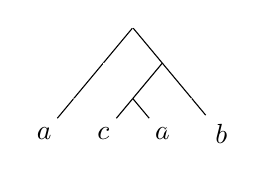
\begin{tikzpicture}[xscale=0.5, yscale=0.3]
      \node[minimum size=0pt, inner sep=0pt] {}
      child {
        child {
          child {node {$a$}}
          child[color=white] {}
        }
        child[color=white] {}
      }
      child {
        child {
          child {node {$c$}}
          child {node {$a$}}
        }
        child {
          child[color=white] {}
          child {node {$b$}}
        }
      };
    \end{tikzpicture}
  \end{equation*}
  which corresponds to the parenthesized product $a \cdot ((c \cdot a) \cdot b)$.
  According to the Cayley table, this product equals $a$.
\end{example}

\begin{lemma}\label{lem:product}
  For any quasigroup on $n$ elements given as a Cayley table, any sequence $(g_0, \dotsc, g_k)$, and any parenthesization $P$ of depth $d$ on that sequence, the parenthesized product $P(g_0, \dotsc, g_k)$ can be computed by an $\L$-uniform family of unbounded fan-in circuits with size $O(k n^2 \log n)$ and depth $O(d)$.
\end{lemma}
\begin{proof}
  How does a circuit access and use a Cayley table for a quasigroup?%
  \footnote{We avoid representing problems using first-order logic, as in the original definition of $\FOLL$ from \autocite{bklm01}, though the logic definition may provide a more natural representation of this sort of information.}
  One way for a circuit to compute the product of two quasigroup elements using the Cayley table is via a multiplexer.
  In the multiplexer, each input has $O(\log n)$ bits, since each quasigroup element can be represented with $O(\log n)$ bits and each input is a pair of quasigroup elements.
  A multiplexer that selects from $n^2$ inputs, each of length $O(\log n)$, can be implemented by an \emph{unbounded fan-in} circuit of depth $O(1)$ and size $O(n^2 \log n)$.
\end{proof}

\subsection{Independent and generating sets}

An element $x$ of a subset $S$ of a magma is \emph{independent with respect to $S$} if $x$ is not in $\gen{S \setminus \{x\}}$.
A subset $S$ is \emph{independent} if each element of $S$ is independent with respect to $S$.

\begin{example}
  In the finite group $C_6$, the cyclic group on six elements, the set $\{g^2, g^3\}$ is independent but the set $\{g^2, g^4\}$ is not independent.
\end{example}

The dual notion of an independent set is that of a generating set.
If $\gen{S} = G$, then $S$ is called a \emph{generating set for $G$}.
The \emph{rank of a magma $G$}, denoted $\rank(G)$, is the minimum cardinality of a generating set.
This terminology extends to semigroups and groups as well.

\begin{example}\label{ex:semigroupgen}
  Consider the right zero semigroup on $n$ elements, a generalization of \autoref{ex:zero}.
  In this semigroup, call it $G$, we have $x \cdot y = y$ for each $x$ and $y$ in $G$.
  The rank of this semigroup must be $n$.
  Assume for the sake of producing a contradiction that the rank is strictly less than $n$.
  Thus there is an element $z$ not in the generating set such that $x_1 \cdot \dotsb \cdot x_n = z$, where each $x_i$ is an element of the generating set.
  This is a contradiction with the fact that $x_1 \cdot \dotsb \cdot x_n = x_n$, since $x_n$ is a right zero.
  Therefore the rank of the semigroup must be $n$.
\end{example}

\begin{example}\label{ex:elementary}
  Consider the elementary abelian $2$-group, $(\mathbb{Z} / 2 \mathbb{Z})^k$, for some positive integer $k$.
  Let $n$ denote the order of this group, so $n = 2^k$.
  The minimum generating set for this group is $\{e_1, \dotsc, e_k\}$, where $e_i$ is the $k$-tuple with a one in the $i$th position and a zero in each other position (if we consider the group as a vector space, $e_i$ is the standard basis vector).
  Thus the group has a minimum generating set of size $k$, which is $\log n$.
\end{example}

For quasigroups, we consider a slightly more specific notion of ``generating''\kern-0.5em.
If $(g_0, \dotsc, g_k)$ is a finite sequence of quasigroup elements denoted $S$ and $P$ is a parenthesization of that sequence, then the \emph{cube of $S$ with respect to $P$}, denoted $\cube_P(S)$, is defined
\begin{equation*}
  \cube_P(S) = \left\{P(g_0, g_1^{\epsilon_1}, \dotsc, g_k^{\epsilon_k}) \, \middle| \, \epsilon_i \in \{0, 1\} \text{ for each } i \right\},
\end{equation*}
where $g_i^{\epsilon_i}$ denotes $g_i$ if $\epsilon_i = 1$ and the empty word if $\epsilon_i = 0$.
The element $g_0$ has no exponent because the empty word by itself is not an element in a quasigroup.
(This is called a ``cube'' because each vertex of the $k$-dimensional Boolean hypercube, when interpreted as a binary string $\epsilon_1 \dotsb \epsilon_k$, yields a quasigroup element.)
If $\cube_P(S) = G$, then $g$ is called a \emph{cube generating sequence of size $k + 1$} for the quasigroup $G$.
The \emph{rank of a quasigroup $G$}, denoted $\rank(G)$, is the minimum size of a cube generating sequence.%
\footnote{
  This is a nonstandard definition of ``rank'' for quasigroups.
  Elsewhere, the rank of a quasigroup is the number of blocks in the partition of the quasigroup into conjugacy classes according to the action of the quasigroup on itself.
}
Contrast the rank of a quasigroup with the rank of a semigroup: the former is the size of a sequence, the latter the size of a set.

%% \begin{example}
%%   \todo{Example of a cube generating sequence for a quasigroup.}
%% \end{example}

Ideally, we would like the notion of rank to be identical for each algebraic structure.
If a quasigroup has a cube generating sequence of size at most $k$, then it has a generating set of size at most $k$, specifically the set of distinct elements from the sequence.
However, we conjecture that for sufficiently large sizes, there is a quasigroup that has a generating set of size strictly less than the size of its minimum cube generating sequence.
If this is incorrect, that is if a small generating set implies a small cube generating sequence, we could use the same definition of rank for all our algebraic structures, simplifying our proofs.

Quasigroups have small cube generating sequences, and groups have small generating sets.
As of this publication, upper bounds on the size of generating sets for semigroups remain the subject of research \autocite{gray14}, although in general, some semigroups of order $n$ have rank $n$ (see \autoref{ex:semigroupgen}).
Magmas have even less structure than semigroups, and hence lack a meaningful upper bound as well.

An upper bound for the minimum size of a generating set for quasigroups can be proven by the probabilistic method.

\begin{lemma}[{\autocite[Theorem~3.3]{ctw13}}]\label{lem:small}
  Each finite quasigroup with $n$ elements has a cube generating sequence of size $O(\log n)$ with a parenthesization of depth $O(\log \log n)$.
\end{lemma}

Since a group is a quasigroup, and since a cube generating sequence induces a generating set, the same upper bound can be applied to groups.
However, a more specific (and constructive) upper bound can be proven inductively by considering cosets of increasing size.
In fact, we can prove a more general lemma bounding the size of independent sets that we will use later as well.

\begin{lemma}\label{lem:magind}
  Suppose $G$ is a finite magma of order $n$ such that for each submagma $H$ and each $x \in G \setminus H$, the cosets $xH$ and $H$ are disjoint.
  Each independent subset of $G$ has size at most $\log n$.
\end{lemma}
\begin{proof}
  Let $S$ be an independent subset of $G$ of cardinality $m$.
  Define the sequence of sets $H_0, \dotsc, H_m$ by
  \begin{align*}
    H_0 & = \emptyset \\
    H_i & = \gen{H_{i - 1} \cup \{x_i\}},
  \end{align*}
  where $x_i$ is the $i$th element of $S$ (in an arbitrary ordering).
  Since each $x_i$ is taken from $S$, an independent set, $x_i \notin \gen{H_{i - 1}}$.
  For each $i \in \{1, \dotsc, m\}$, we have $x_i H_{i - 1}$ and $H_{i - 1}$ are disjoint by hypothesis.
  Thus $|H_i| \geq 2 |H_{i - 1}|$, and by induction $|H_m| \geq 2^m$.
  We conclude that $m \leq \log |H_m| \leq \log |G| = \log n$.
\end{proof}

The disjointness requirement in the previous lemma is fairly strict.
% TODO add the citation: \autocite[Section~I.2]{pflugfelder90}
Neither semigroups (the zero semigroup, for example) nor loops necessarily satisfy it.
Still, a finite group satisfies the hypothesis in the previous lemma, so each independent set of a finite group has size at most $\log n$.
Furthermore, each finite group has an independent \emph{generating} set.

\begin{lemma}
  Each finite group has an independent generating set, and specifically its minimum cardinality generating set is independent.
\end{lemma}
\begin{proof}
  Let $S$ be a generating set of minimum cardinality among all generating sets.
  If $S$ is independent, we are done.
  If $S$ is not independent, then there is an element $x$ in $S$ such that $x \in \gen{S \setminus \{x\}}$.
  But then $\gen{S} = \gen{S \setminus \{x\}}$, a contradiction with the minimality of $S$.
  Therefore the minimum cardinality generating set is independent.
\end{proof}

Combining the previous two lemmas we conclude that the minimum cardinality of a generating set of a finite group is at most $\log n$; \autoref{ex:elementary} gives a group that achieves the upper bound.

\begin{lemma}\label{lem:log}
  If $G$ is a finite group of order $n$ then the minimum cardinality of a generating set is at most $\log n$, with equality when the group is a finite elementary abelian $2$-group.
\end{lemma}

%% \begin{proof}[Proof (expanded from \autocite{arvind07})]
%%   %This proof is an expanded version of the proof from \autocite{arvind07}.
%%   %
%%   Suppose $m$ is the size of the minimum generating set.
%%   Let $H_0 = \gen{e}$, where $e$ is the identity element in $G$.
%%   For each $i \in [m]$, let $H_i = \gen{H_{i - 1} \cup \{x_i\}}$ where $x_i \in G \setminus H_{i - 1}$.
%%   Such an $x_i$ must exist for each $i$ because otherwise we would have some set $H_j$, of size less than $m$, which generates the group $G$; this violates the hypothesis that $m$ is the minimum size of a generating set for $G$.

%%   Now, for each $i \in [m]$, we have $x_i \neq e$, by construction.
%%   Furthermore, the cosets $x_i \gen{H_{i - 1}}$ and $e \gen{H_{i - 1}}$ are disjoint.
%%   If we suppose to the contrary that there is some element $y \in e \gen{H_{i - 1}} \cap x_i \gen{H_{i - 1}}$, then $y = x_i h$ for some $h \in H_{i - 1}$, which implies $x_i = yh^{-1}$, and hence $x_i \in H_{i - 1}$ since both $y$ and $h$ are in $H_{i - 1}$.
%%   This is a contradiction with the hypothesis that $x_i \in (G \setminus H_{i - 1})$.
%%   Therefore $|H_i| \geq 2 |H_{i - 1}|$.
%%   By induction, $|G| = |H_m| \geq 2^m$, which implies $m \leq \log |G| = \log n$.

%%   The equality follows from \autoref{ex:elementary}.
%% \end{proof}
%% \todo{Are there subclasses of semigroups that have logarithmic size generating sets, possibly by a non-constructive existential proof via the probablistic method?
%%   For semigroups, it seems the rank can be computed from the complicated formulas in \autocite{gray14}.}

%% \begin{example}
%%   This lemma is particularly interesting to me with respect to the following example.
%%   \todo{This note doesn't particularly belong here, it should be removed; it's just here so I remember it.}

%%   Let $G$ and $H$ be finite groups of order $m$ and $n$, respectively.
%%   Let $S$ and $T$ be generating sets for $G$ and $H$, respectively.
%%   By the previous lemma, $|S| \leq \log m$ and $|T| \leq \log n$.
%%   Since $S$ and $T$ are generatings sets, $S \times T$ is a generating set for $G \times H$.
%%   But $|S \times T| = |S| |T| \leq (\log m) (\log n)$, whereas $\log |G \times H| = \log |G| |H| = \log |G| + \log |H| = \log m + \log n$.
%%   Thus $G \times H$ has a generating set strictly smaller than $S \times T$, for sufficiently large $m$ and $n$.

%%   This is surprising to me because I would expect the direct product of $G$ and $H$ to behave like the span of two independent spaces.
%%   In graph terms, let $\Cay(G, S)$ and $\Cay(H, T)$ be the Cayley graphs of $G$ and $H$ with edges labeled by elements of $S$ and $T$, respectively.
%%   According to \autocite[Proposition~7]{heydemann97},
%%   \begin{equation*}
%%     \Cay(G \times H, S \times T) = \Cay(G, S) \times \Cay(H, T),
%%   \end{equation*}
%%   where the first $\times$ is the direct product of groups, the second is the Cartesian product of sets, and the third is the tensor product of labeled graphs.
%%   A step in a tensor product graph is like two independent steps in the factor graphs.
%% \end{example}
